\documentclass[12pt]{article}
\usepackage{setspace, graphicx, fullpage, amssymb, amsmath, epsfig, natbib, array, multirow, hyperref}
\usepackage{amsfonts, bm} 
\usepackage{dcolumn}
\usepackage{subfigure, float} 
\usepackage[margin=0.75in]{geometry} 
\usepackage{verbatim}
\usepackage{url}
\usepackage{enumerate}
\newcolumntype{d}[1]{D{.}{.}{#1}} 

\begin{document}
	
	\begin{center}
		Update: 04 January 2017
	\end{center}

Over break I have been working to get our final versions of the functions and data put together. At present, I have been able to get the final House year data, tables, and figures for each of our three sorting algorithms. These tables and figures are found at the end of the update. Further, I have included brief summations of the sorting algorithms we are using in order to form a basis for the appendix.

William had asked me to clean the Senate year data preparation file when we met last week, something I am still working on. Unfortunately, in the process of doing this, I found we our current R script for doing this is causing us to lose a number of observations. Looking deeper into the issue has revealed that our recent datasets for Senator year data are down approximately 30 observations from those we conducted our initial Senate analyses on at an earlier point in the project. Since I have thus far been unable to determine exactly where the error is occurring, I am working to entirely rebuild this item in order to determine where the error is developing.

Additionally, working to sort out the differences between our data and that provided to us from Wiseman revealed a greater number of errors and differences between how we wish to categorize variables on its part than on ours. In particular, the Majority and Minority leadership variables included a number of individuals from each Congress beyond the leader and whip and a greater number of women and Latinos were misclassified than were in our data.

\subsection*{An Overview of Our Sorting Algorithms}

\noindent
\textbf{emIRT Only Algorithm}

Of the three sorting algorithms we employ in this project, this one follows most closely to that of Minozzi and Volden (2013), having two key differences. Both these changes are present in the other algorithms as well.

Most simply, we scale member ideal points with mean 0 rather than mean 5 in order to better follow convention. Additionally, while Minozzi and Volden (2013) used \verb|ideal()| to calculate member ideal points based on votes which the algorithm sorted as non party calls. For this paper we instead use \verb|emIRT()| in order to do this. This function is developed in Imai, Lo, and Olmsted (2015) as a method for calculating nearly identical ideal points to those calculated by the \verb|ideal()| function from the \verb|pscl()| package. The authors solved the underlying functions involved in \verb|ideal()| such that their function, \verb|emIRT()| is able to calculate its ideal points much more rapidly. 

As expected, this method produced highly similar results to those of Minozzi and Volden (2013) in a manner which allowed us to run the algorithms relatively quickly. This reduction in computational strain gave us the ability to seek methods which would better sort votes into calls and noncalls, lowering the number of unsorted votes that Minozzi and Volden (2013) termed ``gray'' votes. We ended up using the two best of these, which we detail below.

\noindent
\textbf{Flip Flop Vote Reassignment Algorithm}

In reviewing the manner in which votes were classified, we found that some votes were switching between the call and noncall classification in subsequent iterations of the algorithm. Since our algorithm uses the noncalls only when calculating ideal points and then reclassifying votes, these were simply repeating a pattern of losing party significance in our model when not used to calculate ideal points as a group but regaining it as soon as soon as they were used for this calculation and the opposite group was not. Dubbing these ``flip flop'' votes, we sought to break up the groups of them such that any effects by their grouping would be broken up. In order to do this, we randomly reassigned all votes that had changed designations at least twice in a row. This did not allow us to classify all votes, but it provided a much better percentage of votes sorted.

\noindent
\textbf{Hybrid Algorithm}

Early on, we developed a simulated annealing function within our algorithm hoping to prevent the sort of problems which ultimately led us to focus on randomly reassigning flip flop votes. After developing the flip flop reassignment version of the algorithm, we decided to combine the methods such that there was random reassignment drawn from all votes which would taper off until the 60th iteration with a random reassignment of ``flip flop'' votes beginning in the 30th. While this method underperformed the ``flip flop'' reassignment at maximizing the number of votes sorted in a number of congresses, overall it proved to be the best at doing so overall. The Hybrid designation comes from the fact that it combines these two methods of reassigning votes in different iterations.

\begin{table}
	\begin{center}
		\begin{tabular}{l c c c c c c }
			\hline
			& Dems 97 & Dems 102 & Dems 107 & Reps 97 & Reps 102 & Reps 107 \\
			\hline
			(Intercept)            & $0.14$       & $-20.24$      & $5.63$        & $12.19^{*}$  & $-30.90^{***}$ & $14.46$       \\
			& $(4.69)$     & $(11.49)$     & $(5.21)$      & $(5.00)$     & $(8.16)$       & $(7.41)$      \\
			ideological\_extremism & $4.67^{***}$ & $14.64^{***}$ & $5.92^{***}$  & $8.82^{***}$ & $6.44^{***}$   & $14.72^{***}$ \\
			& $(0.64)$     & $(2.30)$      & $(0.92)$      & $(0.63)$     & $(1.20)$       & $(1.91)$      \\
			pfrate100              & $0.87^{***}$ & $0.97^{***}$  & $0.84^{***}$  & $0.60^{***}$ & $1.13^{***}$   & $0.49^{***}$  \\
			& $(0.05)$     & $(0.13)$      & $(0.06)$      & $(0.05)$     & $(0.09)$       & $(0.07)$      \\
			dpres                  & $0.04$       & $0.10$        & $0.15^{***}$  & $0.06$       & $0.12$         & $0.35^{***}$  \\
			& $(0.04)$     & $(0.05)$      & $(0.04)$      & $(0.05)$     & $(0.07)$       & $(0.06)$      \\
			south                  & $-1.95^{*}$  & $-4.92^{***}$ & $-0.84$       & $-1.52$      & $2.62^{*}$     & $0.30$        \\
			& $(0.83)$     & $(0.88)$      & $(0.91)$      & $(0.92)$     & $(1.05)$       & $(0.80)$      \\
			votepct                & $-0.02$      & $-0.05$       & $-0.11^{***}$ & $0.08^{*}$   & $-0.00$        & $-0.08^{*}$   \\
			& $(0.03)$     & $(0.03)$      & $(0.03)$      & $(0.04)$     & $(0.03)$       & $(0.04)$      \\
			female                 & $-0.68$      & $0.29$        & $0.26$        & $-2.50$      & $0.11$         & $-1.57$       \\
			& $(1.65)$     & $(1.37)$      & $(0.87)$      & $(1.56)$     & $(1.93)$       & $(1.23)$      \\
			afam                   & $-0.61$      & $-2.23$       & $-1.37$       &              & $0.27$         & $1.54$        \\
			& $(1.71)$     & $(1.76)$      & $(1.23)$      &              & $(5.20)$       & $(5.44)$      \\
			latino                 & $2.02$       & $2.58$        & $-0.09$       & $2.65$       & $-5.30$        & $1.32$        \\
			& $(2.34)$     & $(2.13)$      & $(1.32)$      & $(4.46)$     & $(5.41)$       & $(2.20)$      \\
			seniority              & $-0.08$      & $0.10$        & $-0.14$       & $0.14$       & $0.19$         & $-0.25$       \\
			& $(0.10)$     & $(0.11)$      & $(0.09)$      & $(0.13)$     & $(0.14)$       & $(0.13)$      \\
			freshman               & $-0.75$      & $0.81$        & $-1.85$       & $4.02^{***}$ & $1.89$         & $-2.19$       \\
			& $(1.16)$     & $(1.34)$      & $(1.43)$      & $(1.04)$     & $(1.56)$       & $(1.18)$      \\
			retiree                & $-0.09$      & $0.62$        & $0.40$        & $1.31$       & $-0.30$        & $-2.01$       \\
			& $(1.32)$     & $(1.04)$      & $(1.80)$      & $(1.46)$     & $(1.02)$       & $(1.61)$      \\
			bestgrosswart          & $0.03$       & $0.09$        & $0.20^{**}$   & $0.10$       & $-0.05$        & $0.29^{**}$   \\
			& $(0.07)$     & $(0.09)$      & $(0.07)$      & $(0.07)$     & $(0.11)$       & $(0.10)$      \\
			leader                 & $3.55$       & $-1.96$       & $0.77$        & $0.76$       & $-1.26$        & $-0.70$       \\
			& $(2.31)$     & $(2.26)$      & $(1.72)$      & $(1.89)$     & $(1.94)$       & $(1.85)$      \\
			power                  & $2.13^{*}$   & $1.26$        & $-1.85$       & $-3.09^{**}$ & $0.13$         & $-1.60$       \\
			& $(0.87)$     & $(1.03)$      & $(0.95)$      & $(1.05)$     & $(1.23)$       & $(0.95)$      \\
			chair                  & $2.54^{*}$   & $0.99$        & $2.49$        &              & $0.51$         & $1.39$        \\
			& $(1.22)$     & $(1.53)$      & $(4.92)$      &              & $(5.12)$       & $(1.35)$      \\
			\hline
			R$^2$                  & 0.85         & 0.79          & 0.75          & 0.75         & 0.74           & 0.65          \\
			Adj. R$^2$             & 0.84         & 0.78          & 0.73          & 0.73         & 0.71           & 0.63          \\
			Num. obs.              & 229          & 261           & 207           & 185          & 159            & 211           \\
			RMSE                   & 4.37         & 5.54          & 4.52          & 4.36         & 4.97           & 4.77          \\
			\hline
			\multicolumn{7}{l}{\scriptsize{$^{***}p<0.001$, $^{**}p<0.01$, $^*p<0.05$}}
		\end{tabular}
		\caption{MV 2013 Table 3, emIRT Only Algorithm}
	\end{center}
\end{table}


\begin{table}
	\begin{center}
		\begin{tabular}{l c c c c }
			\hline
			& Democrats & Republicans & Majority & Minority \\
			\hline
			(Intercept)            & $-1.74$       & $-0.29$      & $4.65^{**}$   & $9.16^{***}$  \\
			& $(1.60)$      & $(1.81)$     & $(1.64)$      & $(1.62)$      \\
			ideological\_extremism & $4.76^{***}$  & $6.72^{***}$ & $7.31^{***}$  & $7.49^{***}$  \\
			& $(0.26)$      & $(0.26)$     & $(0.27)$      & $(0.24)$      \\
			pfrate100              & $0.89^{***}$  & $0.71^{***}$ & $0.76^{***}$  & $0.61^{***}$  \\
			& $(0.02)$      & $(0.02)$     & $(0.02)$      & $(0.02)$      \\
			dpres                  & $0.01$        & $0.25^{***}$ & $0.14^{***}$  & $0.23^{***}$  \\
			& $(0.01)$      & $(0.02)$     & $(0.01)$      & $(0.01)$      \\
			south                  & $-3.61^{***}$ & $1.73^{***}$ & $0.64^{**}$   & $-1.73^{***}$ \\
			& $(0.25)$      & $(0.29)$     & $(0.23)$      & $(0.29)$      \\
			votepct                & $0.03^{***}$  & $0.00$       & $-0.01$       & $-0.01$       \\
			& $(0.01)$      & $(0.01)$     & $(0.01)$      & $(0.01)$      \\
			female                 & $0.50$        & $-1.53^{**}$ & $-1.76^{***}$ & $0.75$        \\
			& $(0.35)$      & $(0.49)$     & $(0.41)$      & $(0.41)$      \\
			afam                   & $-0.07$       & $-1.25$      & $-4.06^{***}$ & $-3.65^{***}$ \\
			& $(0.42)$      & $(2.53)$     & $(0.52)$      & $(0.55)$      \\
			latino                 & $-0.90$       & $0.54$       & $-0.75$       & $-2.37^{***}$ \\
			& $(0.51)$      & $(1.02)$     & $(0.64)$      & $(0.65)$      \\
			seniority              & $-0.13^{***}$ & $-0.12^{**}$ & $-0.10^{**}$  & $-0.13^{***}$ \\
			& $(0.03)$      & $(0.04)$     & $(0.03)$      & $(0.04)$      \\
			freshman               & $0.43$        & $0.61$       & $0.34$        & $0.36$        \\
			& $(0.33)$      & $(0.39)$     & $(0.32)$      & $(0.39)$      \\
			retiree                & $-0.55$       & $-0.42$      & $-0.38$       & $-0.82$       \\
			& $(0.45)$      & $(0.52)$     & $(0.44)$      & $(0.53)$      \\
			bestgrosswart          & $0.06^{**}$   & $0.11^{***}$ & $0.08^{**}$   & $0.08^{**}$   \\
			& $(0.02)$      & $(0.03)$     & $(0.02)$      & $(0.03)$      \\
			leader                 & $0.61$        & $1.24$       & $2.32^{***}$  & $1.08$        \\
			& $(0.61)$      & $(0.64)$     & $(0.64)$      & $(0.60)$      \\
			power                  & $1.14^{***}$  & $-0.31$      & $0.50$        & $-0.13$       \\
			& $(0.29)$      & $(0.35)$     & $(0.28)$      & $(0.36)$      \\
			chair                  & $3.23^{***}$  & $2.59^{***}$ & $1.57^{***}$  & $3.88$        \\
			& $(0.46)$      & $(0.67)$     & $(0.41)$      & $(3.75)$      \\
			\hline
			R$^2$                  & 0.73          & 0.62         & 0.72          & 0.61          \\
			Adj. R$^2$             & 0.73          & 0.61         & 0.72          & 0.61          \\
			Num. obs.              & 3982          & 3140         & 4100          & 3022          \\
			RMSE                   & 6.19          & 6.64         & 6.27          & 6.48          \\
			\hline
			\multicolumn{5}{l}{\scriptsize{$^{***}p<0.001$, $^{**}p<0.01$, $^*p<0.05$}}
		\end{tabular}
		\caption{Congresses 93-112, emIRT Only Algorithm}
	\end{center}
\end{table}

\begin{table}
	\begin{center}
		\begin{tabular}{l c c c c c c }
			\hline
			& Dems 97 & Dems 102 & Dems 107 & Reps 97 & Reps 102 & Reps 107 \\
			\hline
            (Intercept)            & $-0.04$      & $-32.76^{**}$ & $-35.81^{***}$ & $12.17^{*}$  & $-31.33^{***}$ & $-16.88^{*}$  \\
            & $(4.66)$     & $(11.88)$     & $(6.58)$       & $(5.00)$     & $(8.10)$       & $(7.91)$      \\
            ideological\_extremism & $4.80^{***}$ & $12.01^{***}$ & $-1.33$        & $8.67^{***}$ & $7.41^{***}$   & $17.87^{***}$ \\
            & $(0.64)$     & $(2.24)$      & $(1.37)$       & $(0.63)$     & $(1.23)$       & $(2.22)$      \\
            pfrate100              & $0.87^{***}$ & $1.12^{***}$  & $1.27^{***}$   & $0.60^{***}$ & $1.11^{***}$   & $0.80^{***}$  \\
            & $(0.05)$     & $(0.13)$      & $(0.08)$       & $(0.05)$     & $(0.09)$       & $(0.08)$      \\
            dpres                  & $0.04$       & $0.14^{*}$    & $0.27^{***}$   & $0.05$       & $0.15^{*}$     & $0.25^{***}$  \\
            & $(0.04)$     & $(0.05)$      & $(0.05)$       & $(0.05)$     & $(0.07)$       & $(0.05)$      \\
            south                  & $-1.82^{*}$  & $-4.03^{***}$ & $-0.24$        & $-1.59$      & $3.10^{**}$    & $1.01$        \\
            & $(0.83)$     & $(0.88)$      & $(1.09)$       & $(0.92)$     & $(1.05)$       & $(0.74)$      \\
            votepct                & $-0.02$      & $-0.06^{*}$   & $-0.13^{**}$   & $0.08^{*}$   & $-0.01$        & $-0.04$       \\
            & $(0.03)$     & $(0.03)$      & $(0.04)$       & $(0.04)$     & $(0.03)$       & $(0.04)$      \\
            female                 & $-0.62$      & $-0.02$       & $2.32^{*}$     & $-2.45$      & $-1.65$        & $-0.93$       \\
            & $(1.64)$     & $(1.38)$      & $(1.06)$       & $(1.57)$     & $(1.91)$       & $(1.16)$      \\
            afam                   & $-0.48$      & $-3.21$       & $-1.49$        &              & $-1.53$        & $-1.35$       \\
            & $(1.70)$     & $(1.78)$      & $(1.50)$       &              & $(5.18)$       & $(5.12)$      \\
            latino                 & $1.96$       & $2.46$        & $-0.95$        & $2.33$       & $-5.05$        & $1.32$        \\
            & $(2.32)$     & $(2.15)$      & $(1.60)$       & $(4.46)$     & $(5.40)$       & $(2.07)$      \\
            seniority              & $-0.09$      & $0.13$        & $0.10$         & $0.13$       & $0.29^{*}$     & $-0.15$       \\
            & $(0.10)$     & $(0.11)$      & $(0.11)$       & $(0.13)$     & $(0.14)$       & $(0.12)$      \\
            freshman               & $-0.76$      & $0.15$        & $-1.89$        & $4.05^{***}$ & $1.46$         & $-1.95$       \\
            & $(1.15)$     & $(1.35)$      & $(1.73)$       & $(1.04)$     & $(1.55)$       & $(1.11)$      \\
            retiree                & $-0.15$      & $0.21$        & $-1.88$        & $1.23$       & $-0.57$        & $-2.68$       \\
            & $(1.31)$     & $(1.05)$      & $(2.19)$       & $(1.46)$     & $(1.02)$       & $(1.52)$      \\
            bestgrosswart          & $0.04$       & $0.12$        & $0.16$         & $0.10$       & $-0.09$        & $0.27^{**}$   \\
            & $(0.07)$     & $(0.09)$      & $(0.09)$       & $(0.07)$     & $(0.11)$       & $(0.09)$      \\
            leader                 & $3.43$       & $-0.55$       & $1.69$         & $0.88$       & $-1.48$        & $0.31$        \\
            & $(2.30)$     & $(2.26)$      & $(2.09)$       & $(1.89)$     & $(1.94)$       & $(1.73)$      \\
            power                  & $2.09^{*}$   & $1.30$        & $-0.19$        & $-3.09^{**}$ & $0.31$         & $-2.13^{*}$   \\
            & $(0.86)$     & $(1.04)$      & $(1.16)$       & $(1.05)$     & $(1.23)$       & $(0.88)$      \\
            chair                  & $2.52^{*}$   & $0.95$        & $0.13$         &              & $1.19$         & $1.01$        \\
            & $(1.22)$     & $(1.54)$      & $(5.99)$       &              & $(5.11)$       & $(1.26)$      \\
            \hline
            R$^2$                  & 0.85         & 0.77          & 0.73           & 0.75         & 0.75           & 0.69          \\
            Adj. R$^2$             & 0.84         & 0.76          & 0.71           & 0.73         & 0.73           & 0.66          \\
            Num. obs.              & 229          & 261           & 207            & 185          & 159            & 211           \\
            RMSE                   & 4.34         & 5.58          & 5.49           & 4.37         & 4.96           & 4.48          \\
            \hline
            \multicolumn{7}{l}{\scriptsize{$^{***}p<0.001$, $^{**}p<0.01$, $^*p<0.05$}}
		\end{tabular}
\caption{MV 2013 Table 3, Flip Flop Reassignment Algorithm}
\end{center}
\end{table}

\begin{table}
	\begin{center}
		\begin{tabular}{l c c c c }
			\hline
            & Democrats & Republicans & Majority & Minority \\
            \hline
            (Intercept)            & $-6.26^{***}$ & $3.38^{*}$    & $5.70^{***}$  & $5.68^{***}$  \\
            & $(1.54)$      & $(1.70)$      & $(1.57)$      & $(1.58)$      \\
            ideological\_extremism & $4.28^{***}$  & $6.82^{***}$  & $7.27^{***}$  & $7.23^{***}$  \\
            & $(0.25)$      & $(0.24)$      & $(0.26)$      & $(0.24)$      \\
            pfrate100              & $0.94^{***}$  & $0.68^{***}$  & $0.76^{***}$  & $0.64^{***}$  \\
            & $(0.02)$      & $(0.01)$      & $(0.02)$      & $(0.02)$      \\
            dpres                  & $0.02^{*}$    & $0.23^{***}$  & $0.11^{***}$  & $0.24^{***}$  \\
            & $(0.01)$      & $(0.01)$      & $(0.01)$      & $(0.01)$      \\
            south                  & $-3.56^{***}$ & $1.73^{***}$  & $0.42$        & $-1.52^{***}$ \\
            & $(0.24)$      & $(0.27)$      & $(0.22)$      & $(0.28)$      \\
            votepct                & $0.03^{***}$  & $-0.00$       & $-0.01$       & $-0.01$       \\
            & $(0.01)$      & $(0.01)$      & $(0.01)$      & $(0.01)$      \\
            female                 & $0.58$        & $-1.63^{***}$ & $-1.61^{***}$ & $0.78^{*}$    \\
            & $(0.34)$      & $(0.46)$      & $(0.39)$      & $(0.39)$      \\
            afam                   & $0.05$        & $-1.89$       & $-3.06^{***}$ & $-3.87^{***}$ \\
            & $(0.40)$      & $(2.38)$      & $(0.50)$      & $(0.54)$      \\
            latino                 & $-0.73$       & $0.63$        & $-0.37$       & $-2.13^{***}$ \\
            & $(0.49)$      & $(0.95)$      & $(0.61)$      & $(0.63)$      \\
            seniority              & $-0.11^{***}$ & $-0.10^{*}$   & $-0.07^{*}$   & $-0.09^{*}$   \\
            & $(0.03)$      & $(0.04)$      & $(0.03)$      & $(0.04)$      \\
            freshman               & $0.54$        & $0.72^{*}$    & $0.47$        & $0.51$        \\
            & $(0.32)$      & $(0.36)$      & $(0.31)$      & $(0.38)$      \\
            retiree                & $-0.73$       & $-0.53$       & $-0.55$       & $-0.97$       \\
            & $(0.43)$      & $(0.48)$      & $(0.42)$      & $(0.51)$      \\
            bestgrosswart          & $0.06^{**}$   & $0.10^{***}$  & $0.06^{**}$   & $0.08^{**}$   \\
            & $(0.02)$      & $(0.03)$      & $(0.02)$      & $(0.03)$      \\
            leader                 & $0.50$        & $1.52^{*}$    & $2.40^{***}$  & $0.97$        \\
            & $(0.58)$      & $(0.60)$      & $(0.61)$      & $(0.58)$      \\
            power                  & $1.16^{***}$  & $-0.19$       & $0.69^{*}$    & $-0.09$       \\
            & $(0.28)$      & $(0.33)$      & $(0.27)$      & $(0.35)$      \\
            chair                  & $3.04^{***}$  & $2.30^{***}$  & $1.52^{***}$  & $1.75$        \\
            & $(0.44)$      & $(0.63)$      & $(0.39)$      & $(3.64)$      \\
            \hline
            R$^2$                  & 0.75          & 0.63          & 0.74          & 0.63          \\
            Adj. R$^2$             & 0.75          & 0.63          & 0.74          & 0.63          \\
            Num. obs.              & 3982          & 3140          & 4100          & 3022          \\
            RMSE                   & 5.92          & 6.23          & 5.96          & 6.28          \\
            \hline
            \multicolumn{5}{l}{\scriptsize{$^{***}p<0.001$, $^{**}p<0.01$, $^*p<0.05$}}
		\end{tabular}
		\caption{Congresses 93-112, Flip Flop Reassignment Algorithm}
	\end{center}
\end{table}

\begin{table}
	\begin{center}
		\begin{tabular}{l c c c c c c }
			\hline
			& Dems 97 & Dems 102 & Dems 107 & Reps 97 & Reps 102 & Reps 107 \\
			\hline
			(Intercept)            & $-0.88$      & $-26.54^{*}$  & $-39.67^{***}$ & $12.94^{**}$ & $-28.64^{***}$ & $-15.43$      \\
			& $(4.61)$     & $(11.81)$     & $(6.68)$       & $(4.93)$     & $(8.04)$       & $(8.06)$      \\
			ideological\_extremism & $4.56^{***}$ & $12.50^{***}$ & $-1.91$        & $8.86^{***}$ & $7.52^{***}$   & $18.59^{***}$ \\
			& $(0.63)$     & $(2.31)$      & $(1.39)$       & $(0.62)$     & $(1.23)$       & $(2.25)$      \\
			pfrate100              & $0.88^{***}$ & $1.05^{***}$  & $1.31^{***}$   & $0.60^{***}$ & $1.07^{***}$   & $0.78^{***}$  \\
			& $(0.05)$     & $(0.13)$      & $(0.08)$       & $(0.05)$     & $(0.09)$       & $(0.08)$      \\
			dpres                  & $0.04$       & $0.13^{*}$    & $0.28^{***}$   & $0.06$       & $0.15^{*}$     & $0.26^{***}$  \\
			& $(0.04)$     & $(0.05)$      & $(0.05)$       & $(0.05)$     & $(0.07)$       & $(0.05)$      \\
			south                  & $-1.90^{*}$  & $-4.15^{***}$ & $-0.13$        & $-1.52$      & $3.20^{**}$    & $0.86$        \\
			& $(0.83)$     & $(0.87)$      & $(1.10)$       & $(0.91)$     & $(1.05)$       & $(0.77)$      \\
			votepct                & $-0.02$      & $-0.06^{*}$   & $-0.13^{**}$   & $0.07$       & $-0.01$        & $-0.04$       \\
			& $(0.03)$     & $(0.03)$      & $(0.04)$       & $(0.04)$     & $(0.03)$       & $(0.04)$      \\
			female                 & $-0.64$      & $0.44$        & $2.29^{*}$     & $-2.37$      & $-1.84$        & $-1.04$       \\
			& $(1.64)$     & $(1.35)$      & $(1.07)$       & $(1.54)$     & $(1.92)$       & $(1.19)$      \\
			afam                   & $-0.60$      & $-2.98$       & $-1.57$        &              & $-1.78$        & $-1.52$       \\
			& $(1.69)$     & $(1.75)$      & $(1.51)$       &              & $(5.22)$       & $(5.25)$      \\
			latino                 & $2.11$       & $2.45$        & $-1.30$        & $2.79$       & $-4.29$        & $1.46$        \\
			& $(2.32)$     & $(2.11)$      & $(1.62)$       & $(4.40)$     & $(5.43)$       & $(2.12)$      \\
			seniority              & $-0.08$      & $0.15$        & $0.10$         & $0.12$       & $0.28^{*}$     & $-0.16$       \\
			& $(0.10)$     & $(0.11)$      & $(0.11)$       & $(0.13)$     & $(0.14)$       & $(0.12)$      \\
			freshman               & $-0.75$      & $0.45$        & $-1.86$        & $4.00^{***}$ & $2.02$         & $-2.00$       \\
			& $(1.15)$     & $(1.32)$      & $(1.75)$       & $(1.02)$     & $(1.56)$       & $(1.14)$      \\
			retiree                & $-0.16$      & $0.22$        & $-1.99$        & $1.17$       & $-0.41$        & $-2.44$       \\
			& $(1.31)$     & $(1.03)$      & $(2.21)$       & $(1.44)$     & $(1.03)$       & $(1.55)$      \\
			bestgrosswart          & $0.04$       & $0.11$        & $0.16$         & $0.09$       & $-0.08$        & $0.27^{**}$   \\
			& $(0.07)$     & $(0.09)$      & $(0.09)$       & $(0.07)$     & $(0.11)$       & $(0.09)$      \\
			leader                 & $3.51$       & $-1.12$       & $1.73$         & $0.92$       & $-1.30$        & $0.07$        \\
			& $(2.30)$     & $(2.21)$      & $(2.11)$       & $(1.86)$     & $(1.95)$       & $(1.78)$      \\
			power                  & $2.01^{*}$   & $1.17$        & $-0.20$        & $-3.13^{**}$ & $0.08$         & $-2.13^{*}$   \\
			& $(0.86)$     & $(1.02)$      & $(1.17)$       & $(1.04)$     & $(1.24)$       & $(0.91)$      \\
			chair                  & $2.61^{*}$   & $0.82$        & $-0.19$        &              & $1.49$         & $0.94$        \\
			& $(1.21)$     & $(1.51)$      & $(6.05)$       &              & $(5.14)$       & $(1.30)$      \\
			\hline
			R$^2$                  & 0.85         & 0.78          & 0.74           & 0.76         & 0.75           & 0.68          \\
			Adj. R$^2$             & 0.84         & 0.76          & 0.72           & 0.74         & 0.72           & 0.66          \\
			Num. obs.              & 229          & 261           & 207            & 185          & 159            & 211           \\
			RMSE                   & 4.33         & 5.47          & 5.55           & 4.31         & 4.99           & 4.59          \\
			\hline
			\multicolumn{7}{l}{\scriptsize{$^{***}p<0.001$, $^{**}p<0.01$, $^*p<0.05$}}
		\end{tabular}
		\caption{MV 2013 Table 3, Hybrid Algorithm}
	\end{center}
\end{table}

\begin{table}
	\begin{center}
		\begin{tabular}{l c c c c }
			\hline
			& Democrats & Republicans & Majority & Minority \\
			\hline
			(Intercept)            & $-5.09^{**}$  & $4.04^{*}$    & $7.45^{***}$  & $5.60^{***}$  \\
			& $(1.56)$      & $(1.70)$      & $(1.57)$      & $(1.59)$      \\
			ideological\_extremism & $4.51^{***}$  & $6.95^{***}$  & $7.48^{***}$  & $7.24^{***}$  \\
			& $(0.25)$      & $(0.24)$      & $(0.25)$      & $(0.23)$      \\
			pfrate100              & $0.93^{***}$  & $0.67^{***}$  & $0.74^{***}$  & $0.64^{***}$  \\
			& $(0.02)$      & $(0.01)$      & $(0.02)$      & $(0.02)$      \\
			dpres                  & $0.02$        & $0.23^{***}$  & $0.11^{***}$  & $0.24^{***}$  \\
			& $(0.01)$      & $(0.01)$      & $(0.01)$      & $(0.01)$      \\
			south                  & $-3.66^{***}$ & $1.71^{***}$  & $0.28$        & $-1.47^{***}$ \\
			& $(0.25)$      & $(0.27)$      & $(0.22)$      & $(0.28)$      \\
			votepct                & $0.03^{***}$  & $-0.00$       & $-0.01$       & $-0.01$       \\
			& $(0.01)$      & $(0.01)$      & $(0.01)$      & $(0.01)$      \\
			female                 & $0.57$        & $-1.71^{***}$ & $-1.60^{***}$ & $0.76$        \\
			& $(0.34)$      & $(0.46)$      & $(0.39)$      & $(0.40)$      \\
			afam                   & $0.09$        & $-1.80$       & $-2.88^{***}$ & $-3.93^{***}$ \\
			& $(0.40)$      & $(2.37)$      & $(0.50)$      & $(0.54)$      \\
			latino                 & $-0.70$       & $0.66$        & $-0.23$       & $-2.18^{***}$ \\
			& $(0.50)$      & $(0.95)$      & $(0.62)$      & $(0.63)$      \\
			seniority              & $-0.11^{***}$ & $-0.10^{*}$   & $-0.07^{*}$   & $-0.10^{**}$  \\
			& $(0.03)$      & $(0.04)$      & $(0.03)$      & $(0.04)$      \\
			freshman               & $0.57$        & $0.76^{*}$    & $0.53$        & $0.51$        \\
			& $(0.32)$      & $(0.36)$      & $(0.31)$      & $(0.38)$      \\
			retiree                & $-0.95^{*}$   & $-0.47$       & $-0.72$       & $-0.96$       \\
			& $(0.44)$      & $(0.48)$      & $(0.42)$      & $(0.51)$      \\
			bestgrosswart          & $0.06^{*}$    & $0.09^{***}$  & $0.05^{*}$    & $0.08^{**}$   \\
			& $(0.02)$      & $(0.03)$      & $(0.02)$      & $(0.03)$      \\
			leader                 & $0.46$        & $1.58^{**}$   & $2.36^{***}$  & $1.04$        \\
			& $(0.59)$      & $(0.60)$      & $(0.61)$      & $(0.58)$      \\
			power                  & $1.18^{***}$  & $-0.15$       & $0.77^{**}$   & $-0.12$       \\
			& $(0.28)$      & $(0.33)$      & $(0.27)$      & $(0.35)$      \\
			chair                  & $3.17^{***}$  & $2.27^{***}$  & $1.53^{***}$  & $1.55$        \\
			& $(0.45)$      & $(0.63)$      & $(0.40)$      & $(3.65)$      \\
			\hline
			R$^2$                  & 0.74          & 0.63          & 0.73          & 0.63          \\
			Adj. R$^2$             & 0.74          & 0.63          & 0.73          & 0.63          \\
			Num. obs.              & 3982          & 3140          & 4100          & 3022          \\
			RMSE                   & 6.02          & 6.21          & 6.05          & 6.30          \\
			\hline
			\multicolumn{5}{l}{\scriptsize{$^{***}p<0.001$, $^{**}p<0.01$, $^*p<0.05$}}
		\end{tabular}
		\caption{Congresses 93-112, Hybrid Algorithm}
	\end{center}
\end{table}

\begin{figure}[h]
	\caption{Figure 2, Ideological Extremism, emIRT Only Algorithm}
	\centering
	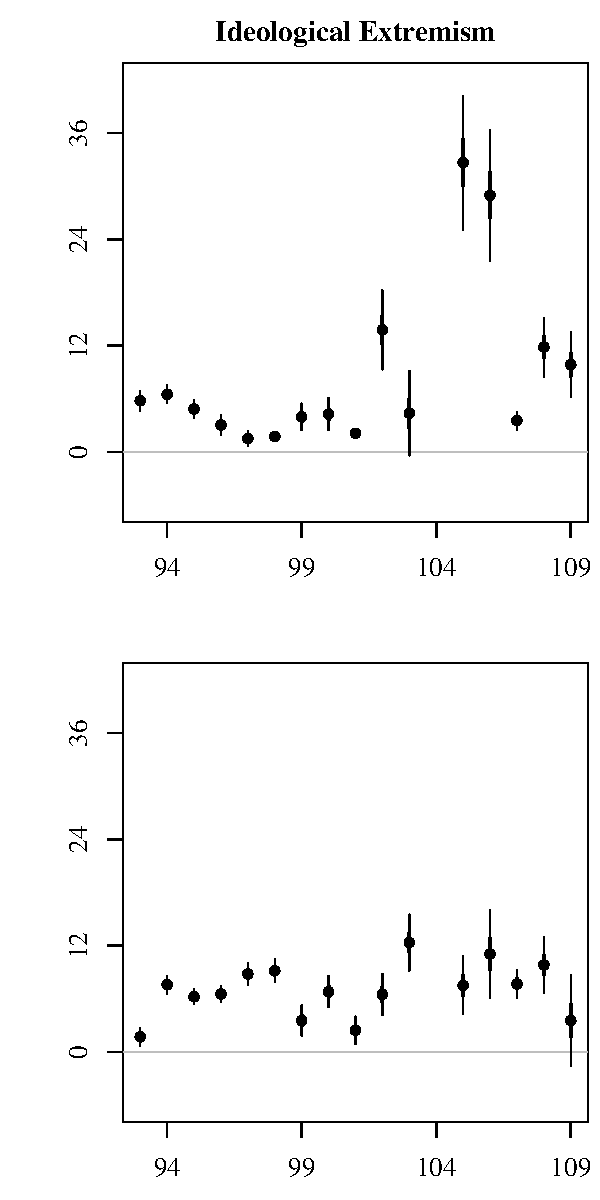
\includegraphics[]{C:/Users/Ethan/Documents/GitHub/partycalls/plots/who-heeds-figure2-replication_emIRT_only.pdf}
	
\end{figure}

\begin{figure}[h]
	\caption{Figure 2, Ideological Extremism, Flip Flop Reassignment Algorithm}
	\centering
	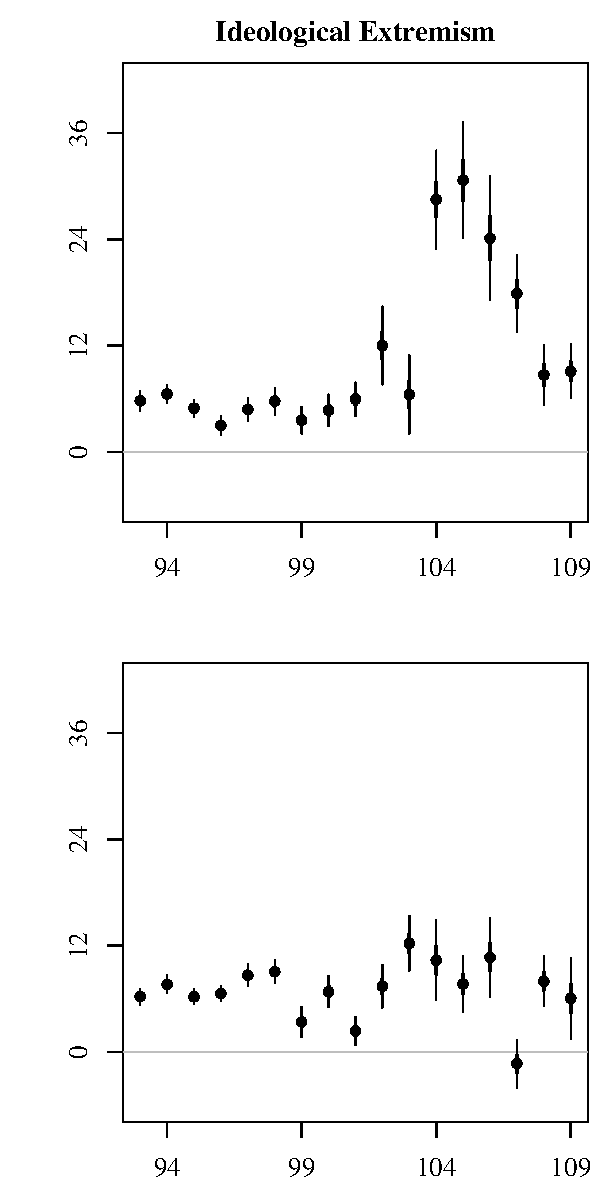
\includegraphics[]{C:/Users/Ethan/Documents/GitHub/partycalls/plots/who-heeds-figure2-replication_reassign_flip_flop.pdf}
	
\end{figure}

\begin{figure}[h]
	\caption{Figure 2, Ideological Extremism, Hybrid Algorithm}
	\centering
	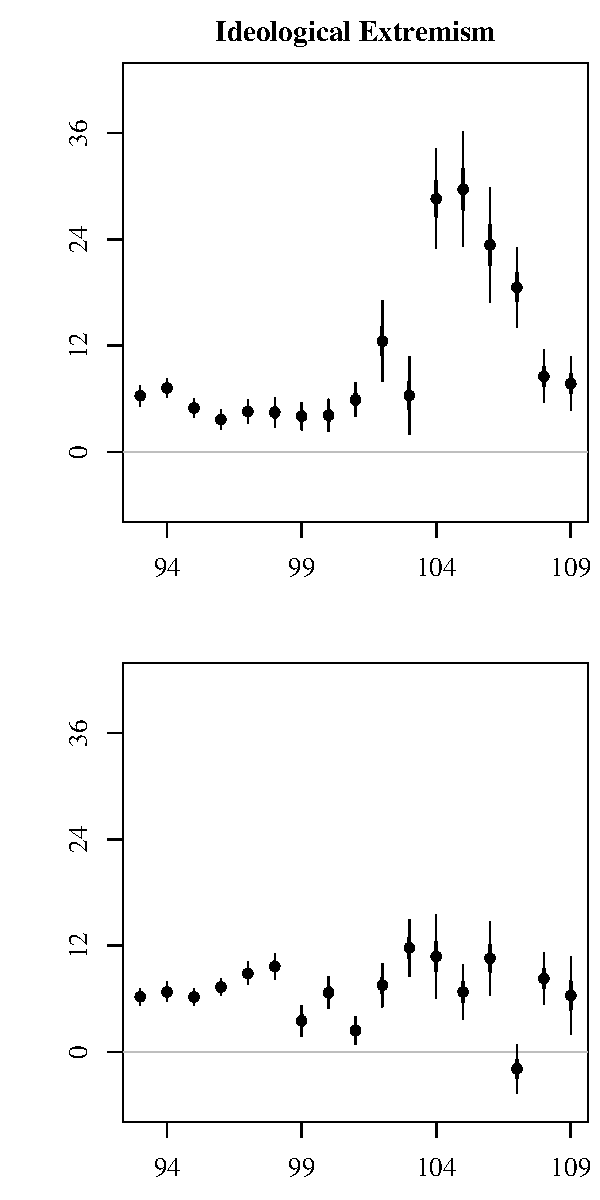
\includegraphics[]{C:/Users/Ethan/Documents/GitHub/partycalls/plots/who-heeds-figure2-replication_hybrid.pdf}
	
\end{figure}
			
			
			
			
			
			

















\end{document}